\subsection{État de l'art}

Les instruments auto-oscillants peuvent être décrits par le couplage entre un excitateur non linéaire auquel le musicien apporte de l'énergie et un résonateur passif linéaire.\cite{mcintyre_oscillations_1983}. Selon le type d'instrument, l'excitateur peut représenter l'archet, le jet d'air causé par le musicien, le mouvement de l'anche. Nous distinguons deux types de modèles physiques permettant la synthèse audio: l'approche modale et l'approche par guide d'ondes.

% J'ai discuté avec Charlotte et du coup on utilise la même fonction non linéaire entre l'article de Taillard et leur approche modale (modélisation de la dynamique de l'anche)

\subsubsection{Approche modale} \label{sec:approche_modale}

\begin{figure}
    \centering
    \includegraphics[scale=.38]{img/schema_chaigne.png}
    \caption{\textit{Schéma du fonctionnement d'un instrument à anche simple \cite{chaigne2008acoustique}.} L'anche étant rectangulaire, le problème peut être décrit en deux dimensions.}
    \label{fig:schema_chaigne}
\end{figure}

Le modèle présenté dans cette partie est tiré de \cite{chaigne2008acoustique}. La figure \ref{fig:schema_chaigne} schématise le fonctionnement d'un instrument à anche simple. La différence de pression entre la bouche du musicien $p_m(t)$ et le canal $p(t)$ induit l'apparition de deux phénomènes : (1) un débit $u(t)$ en sortie de canal ; (2) une force appliquée à l'anche. Dans le cas d'une anche en-dedans (clarinette, saxophone), cette force est dirigée de sorte à diminuer la section à l'entrée du canal. Il existe donc une pression dite "de plaquage statique" $p_M$ pour laquelle l'anche est plaquée contre la partie supérieure du bec. Le débit $u(t)$ à $p_M$ est alors nul. Le mouvement de l'anche induit à son tour l'apparition d'un débit $u_r(t)$ qui s'additionne à $u(t)$. Le débit total à la sortie du canal supérieur est donc $u_{in}(t)=u_r(t)+u(t)$.

Par souci de simplicité, les variables sont exprimées sous forme adimensionnée. Les paramètres de jeu sont définis comme :

\begin{equation}
    \gamma = \frac{p_m}{p_M};\zeta=Z_cwH\sqrt{\frac{2}{\rho p_M}},
\end{equation}\\
où $Z_c$ est l'impédance caractéristique du milieu, $\rho$ est sa masse volumique, $w$ est la largeur effective du canal et $H$ est le déplacement de l'anche au plaquage (voir figure \ref{fig:schema_chaigne}). En néligeant la dynamique de l'anche, l'instrument peut être modélisé par un système à deux équations. La première est :

\begin{equation}
u(t) = \begin{cases}
\zeta(1-\gamma+p)\sqrt{|\gamma-p|} \; sgn(\gamma-p)& \text{si }\gamma-p\geq 1\\
0              & \text{sinon}
\end{cases}.
\label{eq:2eq_1}
\end{equation}\\
En supposant que la pression reste proche de zéro, et que l'anche ne bat pas (ce qui correspond à de faibles valeurs de $\gamma$), l'équation \eqref{eq:2eq_1} peut être approximée par un développement limité :

\begin{equation}
    u = F_0 + Ap + Bp^2 + Cp^3,
\end{equation}\\
où $F_0=\zeta(1-\gamma)\sqrt{\gamma}$ ; $A=\zeta\frac{3\gamma-1}{2\sqrt{\gamma}}$ ; $B=-\zeta\frac{3\gamma+1}{8\gamma^{\frac{3}{2}}}$ ; $C=-\zeta\frac{\gamma+1}{16\gamma^{\frac{5}{2}}}$. Par ailleurs, la pression et le débit sont liés dans le résonateur par la relation d'impédance :

\begin{equation}
    P(\omega)=Z(\omega)U(\omega).
\end{equation}\\
Dans le cas d'un résonateur cylindrique de clarinette, l'impédance normalisée $Z(\omega)$ peut être exprimée analytiquement en fonction de l'impédance de sortie normalisée $Z_s(\omega)$ par la méthode de l'impédance ramenée :

\begin{equation}
    Z(\omega)=\frac{j\tan(kL)+Z_s}{1+j\tan(kL)Z_s(\omega)},
    \label{eq:Z_clari}
\end{equation}\\
où $L$ est la longueur du résonateur. En supposant que la sortie est un piston circulaire de rayon $a$ non bafflé, nous avons :

\begin{equation}
    Z_s(\omega) = \frac{1}{4}(ka)^2+j0.6ka,
    \label{eq:Zs}
\end{equation}\\
où $k$ est le nombre d'onde. L'impédance peut être approchée par décomposition en $N$ modes :

\begin{equation}
    Z(\omega)=j\omega\sum_{n=0}^{N}\frac{F_n}{\omega_n^2-\omega^2+\frac{j\omega\omega_n}{Q_n}},
\end{equation}\\
où $\omega_n$ est la pulsation de la $n^{\text{ème}}$ résonance, $Q_n$ est son facteur de qualité et $F_n$ son facteur modal. Dans le domaine temporel, la pression totale $P$ est donc la somme de ses contributions modales $P_n$ dont l'évolution est décrite par le système couplé de $N$ équations de Van der Pol :

\begin{multline}
    \frac{\text{d}^2}{\text{d}t}p_n(t) + \omega_n^2p_n(t) \;+\\F_n\frac{\text{d}}{\text{d}t}\left[Y_{mn}p_n(t)-Ap(t)-Bp^2(t)-Cp^3(t)\right]=0,
\label{eq:VDP}
\end{multline}\\
où $Y_{mn}$ est la valeur du minimum réel de l'admittance. Remarquons que le couplage provient des termes $p(t)$, issus de la dérivée temporelle du débit total $\frac{\text{d}u}{\text{d}t}$.

\begin{figure}
    \centering
    \begin{subfigure}[b]{.49\linewidth}
        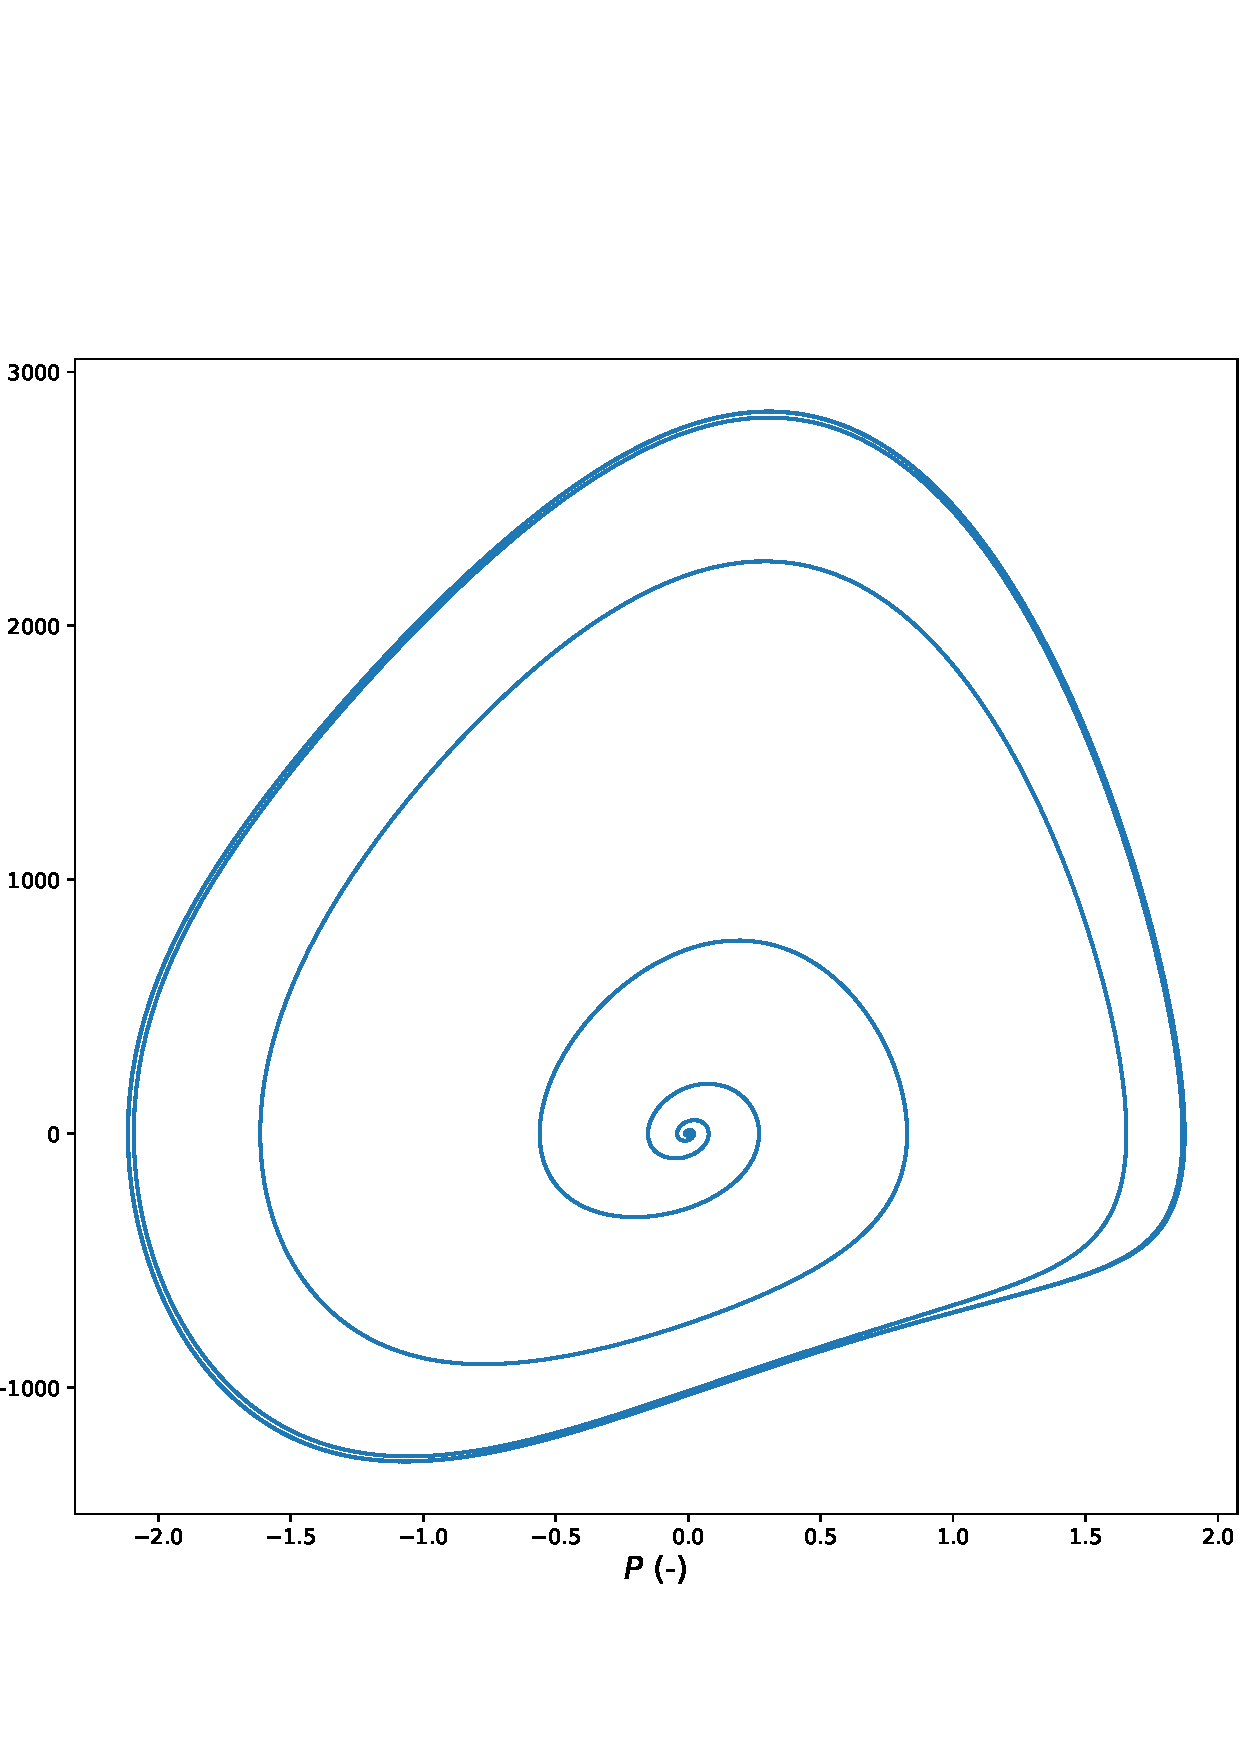
\includegraphics[width=\linewidth]{img/phase_diagram_N1.pdf}
        \caption{$N=1$}
        \label{fig:VDP_phase_N1}
    \end{subfigure}
    \hfill
    \begin{subfigure}[b]{.49\linewidth}
        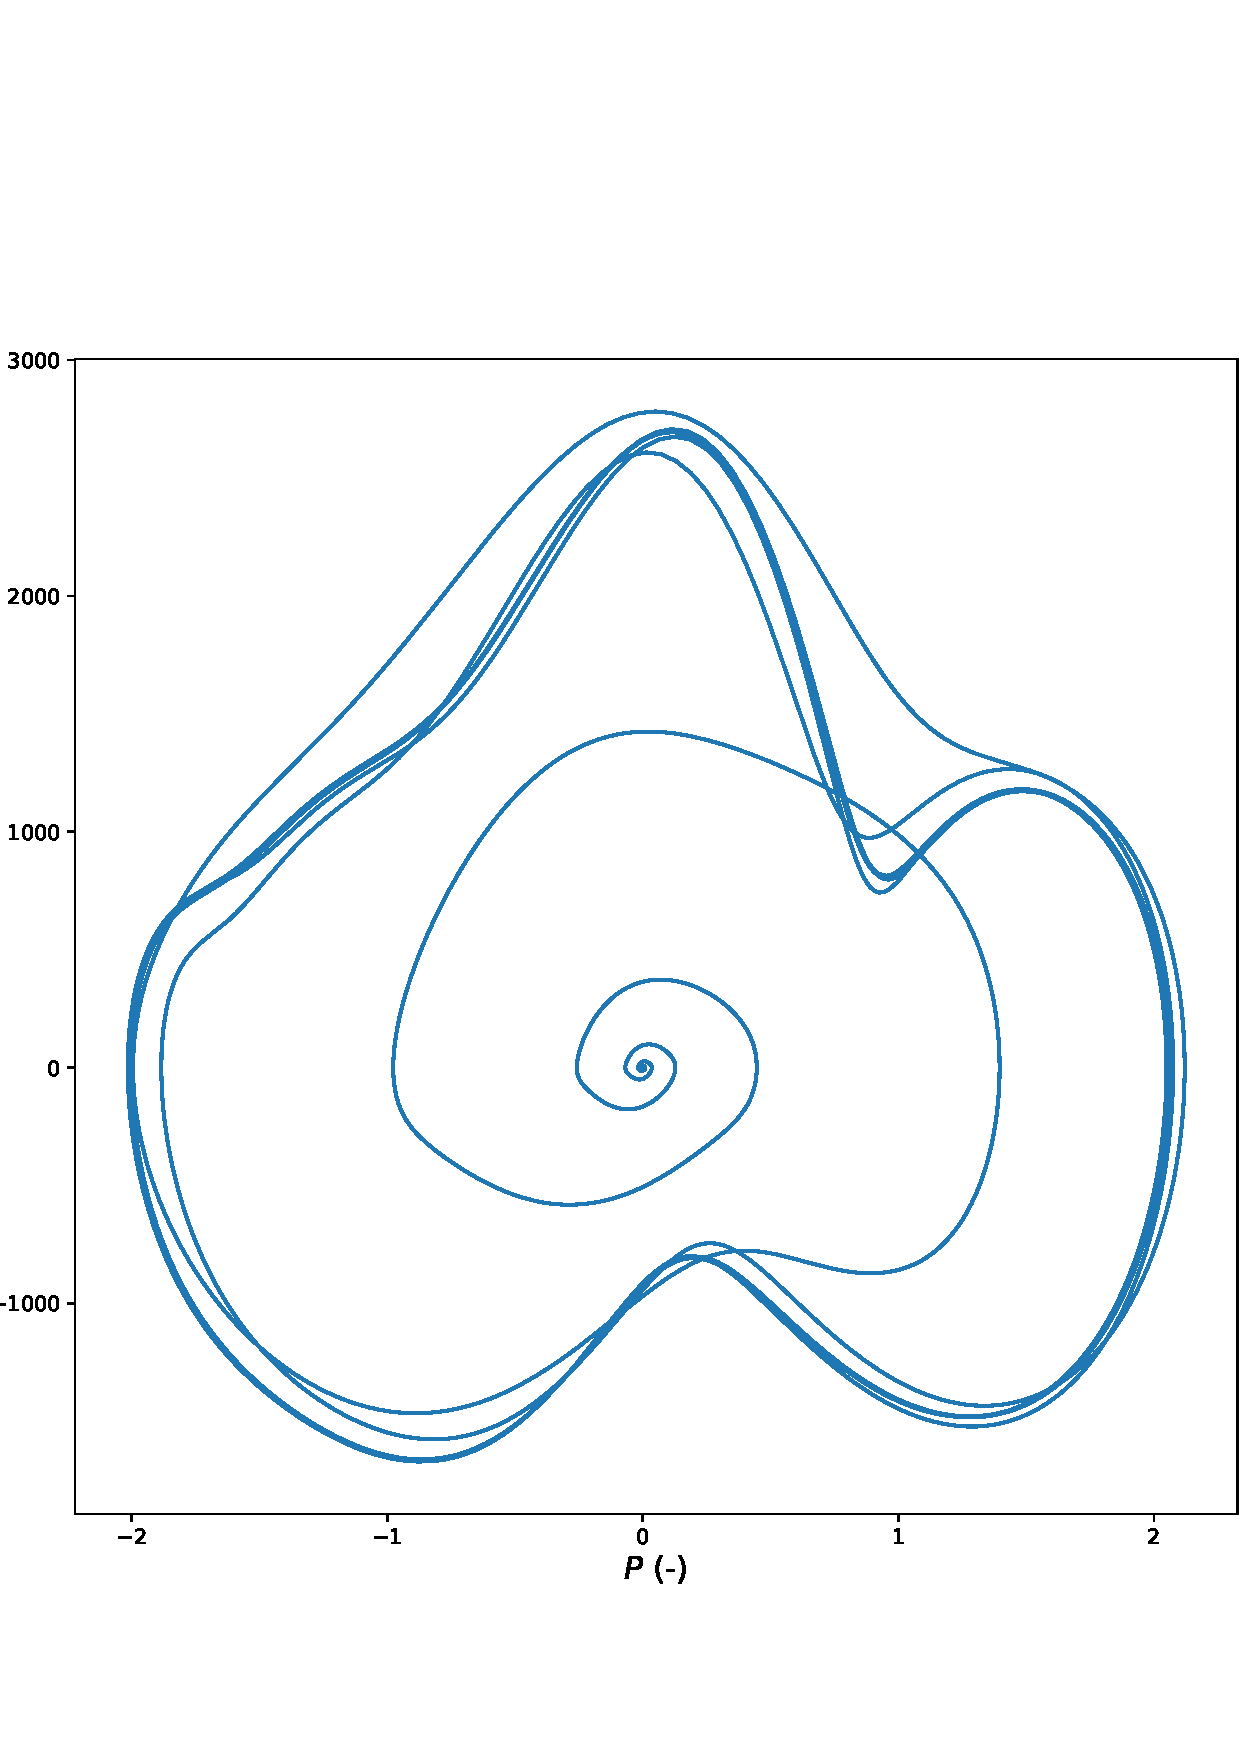
\includegraphics[width=\linewidth]{img/phase_diagram_N2.pdf}
        \caption{$N=2$}
        \label{fig:VDP_phase_N2}
    \end{subfigure}
    \hfill
    \begin{subfigure}[b]{.49\linewidth}
        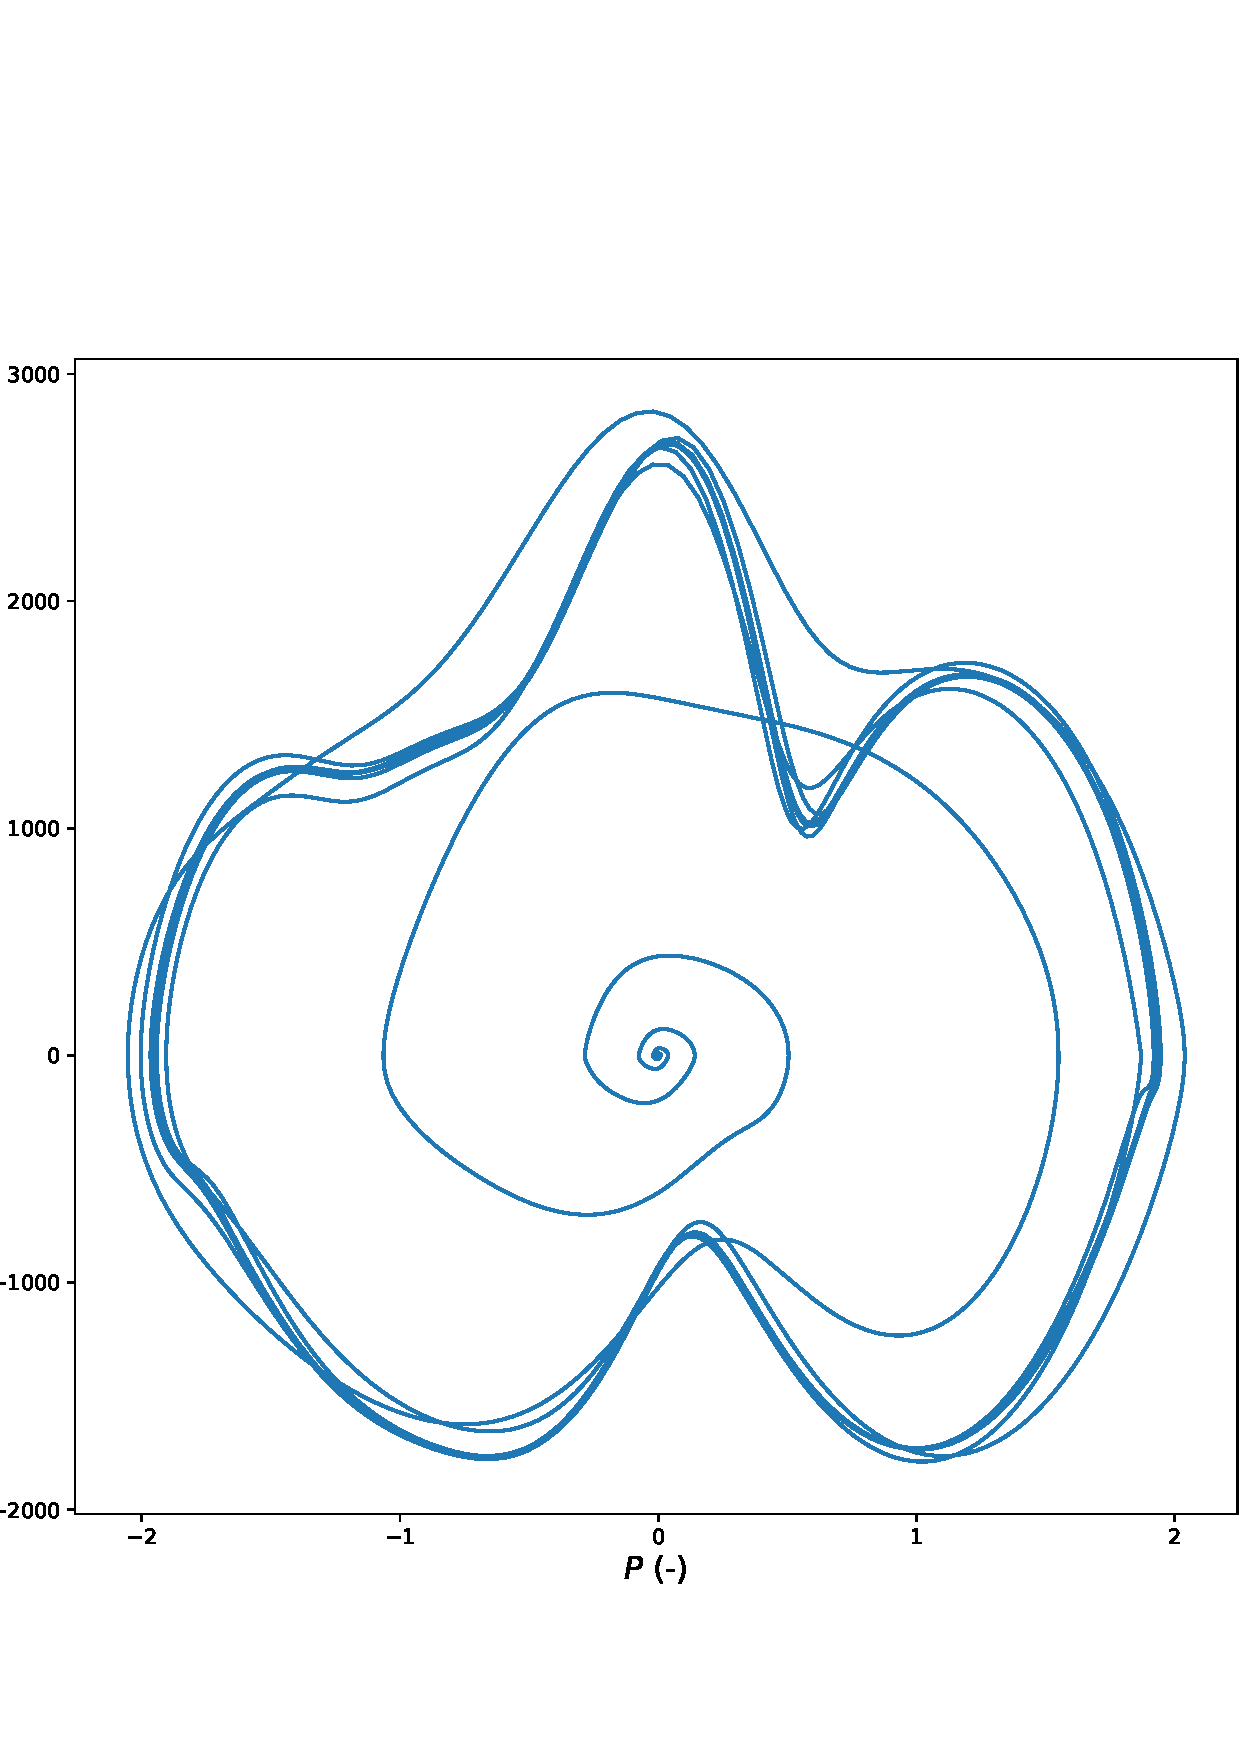
\includegraphics[width=\linewidth]{img/phase_diagram_N3.pdf}
        \caption{$N=3$}
        \label{fig:VDP_phase_N3}
    \end{subfigure}
    \hfill
    \begin{subfigure}[b]{.49\linewidth}
        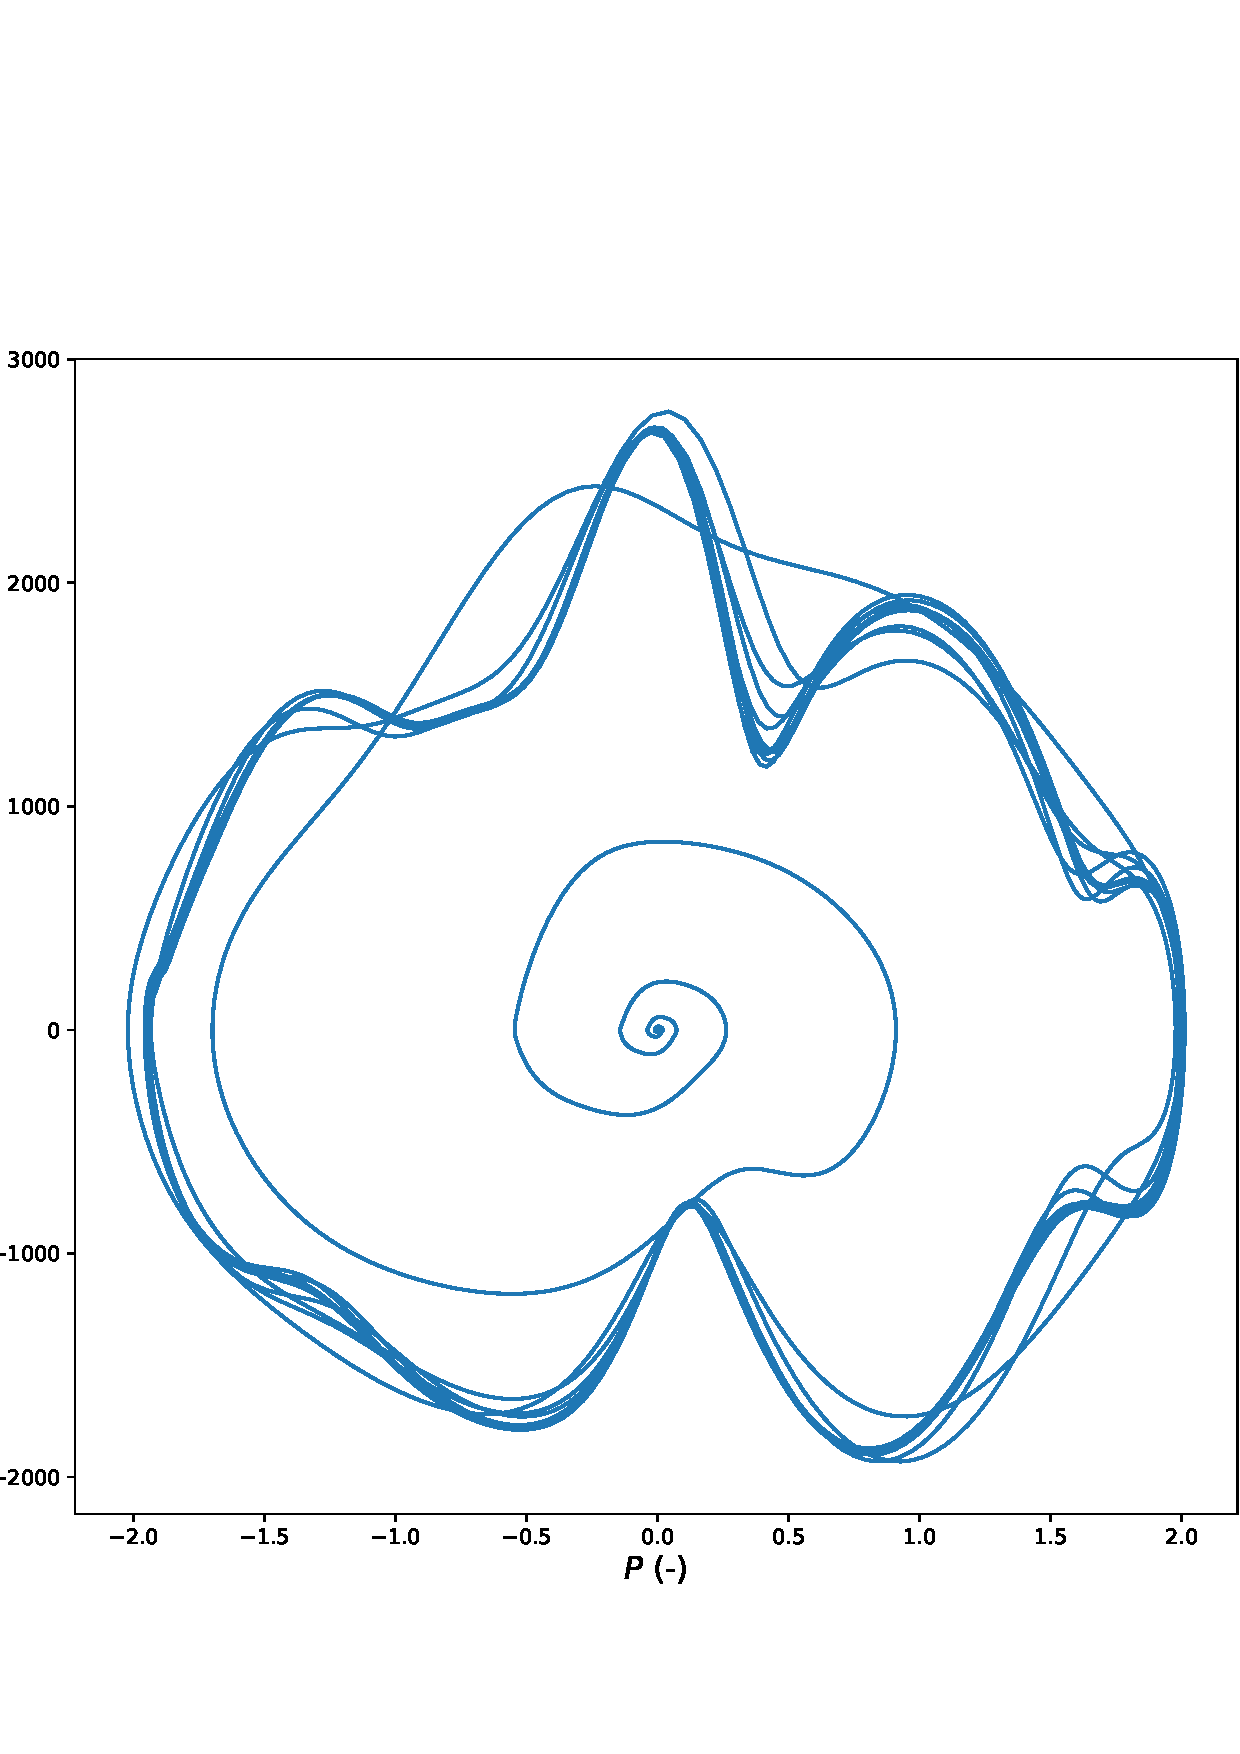
\includegraphics[width=\linewidth]{img/phase_diagram_N4.pdf}
        \caption{$N=4$}
        \label{fig:VDP_phase_N4}
    \end{subfigure}
    \caption{\emph{Evolution du flot $(P_0,\frac{\partial P_0}{\partial t})$ dans l'espace des phases durant l'attaque ($t<0.3$ s) pour $N$ modes.} Le système est initialement perturbé par un saut de pression $P(t=0)=\varepsilon$ ($\varepsilon \ll 1$). Les solutions du système d'équations de Van der Pol convergent vers un cycle limite, dont la forme se complexifie avec N.}
    \label{fig:VDP_phase}
\end{figure}

Dans le cadre de ce projet, nous nous limitons à deux types de solutions : (1) le cas statique $p_n=0$ ; (2) le cas périodique $p_n=\sum_ke^{ik\omega_nt}$. Selon les valeurs des paramètres de jeu $(\gamma,\zeta)$, l'une ou l'autre de ces solutions apparaît. La figure \ref{fig:VDP_phase} montre l'évolution sur $0.3$s du flot dans l'espace des phases $(P_1, \frac{\text{d}P_1}{\text{d}t})$ pour les conditions initiales $p_n(0)=\epsilon$ ($\epsilon\ll1$) et $\frac{\text{d}P}{\text{d}t}=0$. $(\gamma,\zeta)$ est maintenu constant à $(0.7,0.5)$. Nous observons que la perturbation $\epsilon$ du système conduit à la croissance de la pression et de sa dérivée. Le point fixe $(0,0)$ est donc instable. Le flot converge vers un cycle limite stable et correspond à la solution périodique évoquée plus tôt.

En situation réelle de jeu, le couple $(\gamma, \zeta)$ évolue dans le temps pour deux raisons : (1) l'instrumentiste étant un humain, il lui est impossible de maintenir un souffle et une contraction musculaire exactement constants dans le temps ; (2) l'évolution dynamique du son étant au centre de la pratique musicale, la majorité des oeuvres nécessitent une évolution temporelle des paramètres de jeu. Celle-ci a une influence sur la stabilité des solutions (statique en $(0,0)$ ou cycle limite) mais aussi sur l'amplitude et la fréquence des sons joués. Une description des caractéristiques du son joué en fonction des paramètres de jeu est réalisée en partie \ref{sec:descripteurs}. 

L'influence du nombre de modes est visible en figure \ref{fig:VDP_phase}. Le système d'équations \eqref{eq:VDP} étant couplé, chaque mode a une influence sur les autres. Celle-ci est visible par la déformation du cycle limite pour $(P_1, \frac{\text{d}P}{\text{d}t})$, ce qui se traduit par un changement des fréquences de la solution périodique. 


\subsubsection{Approche guide d'ondes}

Le modèle de guide d'ondes sur lequel se base la littérature est celui formulé par McIntyre et al. dans \cite{mcintyre_oscillations_1983}. Dans le cas de la clarinette, la pression et le débit à l'intérieur du résonateur sont séparés en ondes aller et retour. 
A l'aide d'une fonction de réflexion qui peut être déduite de l'impédance d'entrée du résonateur, on peut alors exprimer l'onde retour en fonction de l'onde aller : $p^-(t) = [r * p^+] (t)$.

Différentes simplifications peuvent être effectuées : en supposant l'impédance de rayonnement nulle, on trouve $r(t) = - \delta(t-T)$ avec $T = 2L/c$ le temps d'aller-retour de l'onde dans le résonateur \cite{taillardIteratedMapsClarinetlike2010}. Ce modèle est cependant trop simpliste car il ne tient pas compte des pertes. Le modèle de Raman, initialement conçu pour les cordes frottées \cite{raman1918mechanical} est donc préféré, y compris pour les instruments à vents comme la clarinette \cite{maganza_bifurcations_1986}. Ce modèle
, incluant simplement un coefficient de réflexion $\lambda$ compris entre 0 et 1,
déduit d'une impédance de rayonnement valant $\varepsilon Z_c$, 
permet d'inclure des pertes constantes en fréquences, mais ne tient pas compte d'une possible dispersion à l'extrémité du résonateur. En reparamétrisant la fonction non linéaire de l'excitateur afin d'exprimer l'onde aller en fonction de l'onde retour, on peut aboutir à une construction géométrique simple du signal de pression, appelé carte itérée \cite{taillardIteratedMapsClarinetlike2010}, dont la fonction d'itération est illustrée en figure \ref{fig:iteration-func}.

\begin{figure}
    \centering
    \includegraphics[width=1\linewidth]{img/iteration_function.pdf}
    \caption{\textit{Fonction d'itération d'une carte itérée pour $\gamma = 0,43$, $\zeta=0,8$ et différentes valeurs de $\lambda$.} Formule analytique de la fonction d'itération tirée de
    \cite{taillardIteratedMapsClarinetlike2010}.}
    \label{fig:iteration-func}
\end{figure}

Bien que le son produit par un tel modèle ait un timbre non réaliste, puisque le modèle présuppose l'existence d'ondes carrées et ne tient pas compte de la géométrie, il permet une étude simple des différents régimes d'oscillations, et d'observer notamment des doublements de période successifs jusqu'au chaos
\cite{bergeotNaissanceOscillationsDans}. Ce phénomène a été étudié d'abord théoriquement puis expérimentalement par \cite{maganza_bifurcations_1986}, qui l'ont observé avec une excitation non-linéaire contrôlée à l'aide d'un circuit analogique. L'étude des itérées d'ordre $2^n$ permet d'analyser la stabilité des régimes dont la période a été doublée $n$ fois \cite{taillardIteratedMapsClarinetlike2010}.

Afin d'obtenir un timbre plus réaliste, on peut utiliser une fonction de réflexion obtenue à partir d'une impédance de rayonnement plus élaborée (modèle du piston plan ou d'un tuyau large \cite{chaigne2008acoustique}), et la méthode de l'impédance ramenée. \cite{mcintyre_oscillations_1983} utilise en première approximation une gaussienne retardée, dont la largeur s'adapte en fonction de la longueur du résonateur. Ceci à le rôle d'un passe-bas, illustrant les pertes plus importantes en hautes fréquences. Afin de gagner en réalisme, on peut ajouter d'autres gaussiennes avec un retard différent pour tenir compte de réflexions multiples.
Ces complexifications rendent cependant inutilisable le schéma de carte itérée avec une simple fonction d'itération prenant en compte à la fois le résonateur et l'excitateur.

% Selon l'instrument modélisé, différentes fonctions de réflexion peuvent être utilisées

% Fonction de réflexion :

% - dirac

% - modèle de Raman \cite{raman1918mechanical}

% - tenir compte de la sélectivité en fréquences des pertes et de la dispersion : modèle

% A l'extrémité ouverte de l'instrument, l'onde retour 

Ces modèles sont également valables avec les instruments à cordes frottées \cite{ollivier_idealized_2004} en effectuant plusieurs analogies entre les grandeurs physiques propres aux instruments à vents (débit et pression), à celles propres aux instruments à cordes frottées (force au point de jeu et vitesse de la corde).

\paragraph{Fonction non linéaire}

Selon l'instrument modélisé et le degré de réalisme visé, différentes fonctions non-linéaires peuvent être utilisées pour modéliser l'excitateur. \cite{mcintyre_oscillations_1983} utilisent une fonction cubique pour tenir compte de l'asymétrie de la courbe d'excitation, plus pentue vers $p=\gamma$ que vers $p=1$. Une fonction cubique est aussi utilisée dans les expériences de \cite{maganza_bifurcations_1986}. Plus récemment, \cite{taillardIteratedMapsClarinetlike2010} ont utilisé l'équation \eqref{eq:2eq_1}.

% \begin{itemize}
%     \item Parabole \cite{mcintyre_oscillations_1983}
%     \item $x^3 - x$ \cite{maganza_bifurcations_1986} utilisé expérimentalement
%     \item Fonction de Kergomard 
% \end{itemize}




\subsection{Méthodes et résultats}

On s'intéresse à comparer ces deux approches de modélisation de ces instrument, en terme d'intérêt pour la synthèse sonore, capacité prédictive, différents régimes obtenus, et à explorer l'espace de contrôle. 

\subsubsection{Approche modale}\label{sec:result_modal}

Dans un premier temps, l'approche modale nécessite le calcul de l'impédance normalisée $Z(\omega)$ à l'entrée du résonateur. Pour le cas cylindrique de la clarinette, l'expression analytique \eqref{eq:Z_clari} peut directement être utilisée. L'impédance obtenue analytiquement est montrée en figure \ref{fig:Z_clarinette}. Nous observons que la forme analytique est composée de pics distincts à des harmoniques impaires, ce qui est caractéristique de la géométrie cylindre. De plus, la fréquence fondamentale est $138$Hz, ce qui correspond à la note Do\#2. Cela est cohérent avec le registre de la clarinette.

\begin{figure}
    \centering
    \includegraphics[scale=.2]{img/Z_clari.pdf}
    \caption{\emph{Impédances d'un résonateur cylindre de longueur $L=60$cm}. Nous observons que la forme analytique est composée de pics distincts à des harmoniques impaires, ce qui est caractéristique de la géométrie cylindre. De plus, la fréquence fondamentale est $138$Hz, ce qui correspond à la note Do\#2. Cela est cohérent avec le registre de la clarinette.}
    \label{fig:Z_clarinette}
\end{figure}

Pour des géométries plus complexes, la bibliothèque Python OpenWind \cite{ernoult:hal-04217988} développée par l'Inria est utilisée. Celle-ci calcule les impédances par la méthode des éléments finis et des matrices de transfert.

Le système de $N$ équations modales \eqref{eq:VDP} est résolu par la méthode Runge-Kutta d'ordre 4 \cite{butcher1996history}. La représentation d'état suivante est utilisée :

\begin{equation}
    X=\begin{pmatrix}
        P_1\\...\\P_N\\\frac{\text{d}P_1}{\text{d}t}\\...\\\frac{\text{d}P_N}{\text{d}t}
    \end{pmatrix} = \begin{pmatrix}
    x_1\\...\\x_N\\x_{N+1}\\...\\x_{2N}
    \end{pmatrix}.
\end{equation}\\
L'équation dynamique est alors :

\begin{equation}
\begin{split}
    \frac{\text{d}X}{\text{d}t} &= f(X) \\
    &= \begin{pmatrix}
        x_{N+1}\\
        x_{N+2}\\
        ...\\
        x_{2N}\\
        -\omega_1^2x_1-F_1Y_{m1}x_{N+1}+2F_1Bx_s\frac{\text{d}x_s}{\text{d}t}+\\
        3F_1Cx_s^2\frac{\text{d}x_s}{\text{d}t}+F_1A\frac{\text{d}x_s}{\text{d}t}\\
        ...\\
        -\omega_N^2x_N-F_NY_{mN}x_{2N}+2F_NBx_s\frac{\text{d}x_N}{\text{d}t}+\\
        3F_NCx_s^2\frac{\text{d}x_s}{\text{d}t}+F_NA\frac{\text{d}x_s}{\text{d}t}
    \end{pmatrix}
\end{split},
\end{equation}\\
avec $x_s=\sum_{i=1}^Nx_i$ et $\frac{\text{d}x_s}{\text{d}t}=\sum_{i=N+1}^{2N}x_i$. Pour la discrétisation, les coefficients de la méthode Runge-Kutta sont calculés à chaque pas de temps $n$ : 

\begin{equation}
\left\{
    \begin{split}
        K_{1,n} &= T_ef(X_n)\\
        K_{2,n} &= T_ef(X_n+\frac{1}{2}K_{1,n})\\
        K_{3,n} &= T_ef(X_n+\frac{1}{2}K_{2,n})\\
        K_{4,n} &= T_ef(X_n+K_{3,n})
    \end{split}\quad ,
    \right.
\end{equation}\\
où $T_e=\frac{1}{44100}$s est la période d'échantillonnage du signal discrétisé. Cela permet d'approximer l'état au pas de temps suivant :

\begin{equation}
    X_{n+1} = X_n+\frac{1}{6}\left(K_{1,n}+2K_{2,n}+2K_{3,n}+K_{4,n}\right).
\end{equation}

Cette méthode a pour avantage sa facilité d'implémentation. De plus, aucune instabilité n'a été rencontrée lors de nos expériences. Par ailleurs, les résultats obtenus, visibles en figure \ref{fig:VDP_phase}, sont cohérents avec la théorie des oscillateurs de Van der Pol. Enfin, cette méthode a pour avantage son implémentation directe dans un logiciel spécialisé dans le temps réel (dans le cas de ce projet, il s'agit de Max/MSP).

\subsubsection{Cartes itérées}

\begin{figure}[h!]
    \centering
    \begin{subfigure}[b]{.8\linewidth}
        \includegraphics[width=\linewidth]{img/doublement_periode_pressure.pdf}
        \caption{Pression}
        \label{fig:pression doublement periode}
    \end{subfigure}
    % \hfill
    \begin{subfigure}[b]{.8\linewidth}
        \includegraphics[width=\linewidth]{img/doublement_periode_spectre.pdf}
        \caption{Spectre du régime permanent}
        \label{fig:spectre doublement periode}
    \end{subfigure}
    \caption{\emph{Quadruplement de période pour $\zeta=0,8$, $\gamma=0,44$ et $\lambda = 0,95$.} La transformée de Fourier permet uniquement d'observer une multiplication par 2 et non par 4 de la période.}
    \label{fig:doublement periode}
\end{figure}
Un des buts du projet étant de pouvoir jouer différents régimes de la clarinette pour offrir un maximum de variété au musicien, un modèle de Raman a été implémenté en Python puis en temps réel, avec la méthode des cartes itérées (voir la fonction d'itération figure \ref{fig:iteration-func}). En effet, ce modèle nous a permis de constater l'apparition de doublement de période successifs décrits dans \cite{maganza_bifurcations_1986} et \cite{taillardIteratedMapsClarinetlike2010}, particulièrement visibles dans l'espace des phases (voir section \ref{par:espace de phase}). L'observation des paramètres de jeu $\gamma$ et $\zeta$ pour lesquels ces changements de régime ont lieu pouvait être un indicateur pour chercher des régimes similaires avec d'autres modèles plus réalistes.

Afin de se rapprocher d'un son de clarinette, la fonction non-linéaire utilisée est donnée dans l'équation \eqref{eq:2eq_1}. On observe dans la figure \ref{fig:doublement periode} la transition vers un régime avec un quadruplement de période : au lieu d'osciller entre deux valeurs comme elle le fait par exemple pour $\gamma=0,35$, la pression oscille entre huit valeurs. Le résultat perçu est celui de la superposition de la hauteur attendue à $\SI{430}{\Hz}$, et d'un son plus grave, résultant des doublements successifs de période.

Cependant, pour ces paramètres de jeu, le signal produit avec le modèle avec l'approche modale ne comporte pas de doublement de période.
% INSERER RESULTAT AVEC DOUBLEMENT DE PERIODE ET IDEM POUR LES MEMES PARAMS AVEC L'APPROCHE MODALE (ça montrera que malheureusement les modèles diffèrent donc pas possible d'effectuer un transfert aussi rapide)



\subsubsection{Guide d'onde}

Le timbre obtenu par l'approche des cartes itérées avec un simple retard comme fonction de réflexion ne produit par nature pas un timbre réaliste. On implémente également dans Max/MSP une méthode avec ligne à retard et une fonction de réflexion plus complexe.

On teste avec cette implémentation différentes fonctions de réflexion :
\begin{itemize}
    \item Fonction de réflexion issue du calcul de l'impédance de rayonnement d'un piston circulaire non bafflé \eqref{eq:Zs} et de la méthode de l'impédance ramenée
    \item Passe-bas d'ordre 2 à réponse impulsionnelle infinie en s'inspirant de la gaussienne utilisée dans \cite{mcintyre_oscillations_1983}.
\end{itemize}

La première solution donne des résultats peu concluants (explosion de la pression et timbre non réaliste). 

Le filtre passe-bas, avec l'ajout d'une $\tanh$ à la fonction de non linéarité pour contrer le phénomène d'instabilité du modèle engendrant une explosion de la pression, permet lui d'obtenir des résultats plus intéressants. Il est possible pour certains paramètres du filtre d'obtenir un timbre plus proche de celui d'une clarinette. En modifiant les paramètres, on peut s'éloigner du timbre de la clarinette, mais produire des sons qui ont un intérêt musical.

% Ligne à retard, complexification du modèle pour tenir compte des pertes plus importantes en hautes fréquences.